\documentclass[12pt, a4paper, oneside]{ctexbook}
\usepackage{amsmath, amsthm, amssymb, bm, graphicx, hyperref, mathrsfs}
\usepackage{geometry}
\usepackage{subfigure}
\usepackage{pdfpages}
\usepackage{hyperref}[colorlinks=true,linkcolor=black,citecolor=blue,urlcolor=blue]
\usepackage{listings}
%设置引用格式
\hypersetup{
	colorlinks=true,linkcolor=black,colorlinks=true,linkcolor=black,citecolor=blue,urlcolor=blue
}
%在LateX中,参考文献的引用一般有两种方式,平 齐 时 用 命 令\cite{...}, 上 标 时用\textsuperscript{\cite{...}}

\CTEXsetup[format={\Large\bfseries}]{section}	%section 居左(默认居中)
\CTEXsetup[format={\huge\bfseries}]{chapter}	%chapter 居左(默认居中)

%配置纸张边缘
\geometry{left=2.54cm,right=2.54cm,top=3.18cm,bottom=3.18cm}

\title{{\Huge{\textbf{作品介绍论文}}}\normalsize{\\——第六届全国大学生集成电路创新创业大赛景嘉微杯全国总决赛作品介绍论文}}
\author{队名:虹ヶ咲学园芯片设计同好会\\ 成员:黄金源\space邓立唯\space林明锋}
\date{\today}
\linespread{1.5}


\begin{document}
	
	
\includepdf[page=1]{./pic/cover.pdf}
	
	%-----------------------封面------------------
	\maketitle	
	\pagenumbering{Roman}
	\setcounter{page}{1}
	%-----------------------前言------------------
	\begin{center}
		\Huge\textbf{前言}
	\end{center}~\
	
	本文档(作品介绍论文)仅作为虹ヶ咲学园芯片设计同好会(成员:黄金源、邓立唯、林明锋)参加第六届全国大学生集成电路创新创业大赛景嘉微杯赛全国总决赛供组委会展示使用。
	~\\
	\begin{flushright}
		\includegraphics[width=0.25\linewidth]{pic/logo}\\
		\begin{tabular}{c}
			虹ヶ咲学园芯片设计同好会\\
			\today
		\end{tabular}
	\end{flushright}
	%-----------------------目录------------------
	\newpage
	\pagenumbering{Roman}	%Roman or arabic
	\setcounter{page}{1}
	\tableofcontents
	\newpage
	\setcounter{page}{1}
	\pagenumbering{arabic}
	
	%-----------------------正文----------------	
	\chapter{作品介绍}
	\section{背景介绍与赛题分析}
	单幅图像超分辨率重建是指将一副低分辨率图像通过特定算法处理获得高分辨率图像的的一种技术。
	
	图像超分辨率重建一直以来都是图像处理领域中一个重要的研究方向之一,在医学、遥感、图像识别、网络媒体传输、动画制作与合成等领域都有着重要的应用。
	目前已有许多优秀的算法应用于现实的产品上,但是有效保持图像纹理细节且使图像边缘区域不失真,同时兼顾处理速度一直是图像超分辨率重建技术的一个难题。
	\par 在 GPU 处理领域,为了减轻像素引擎的负载,通常使用渲染低分辨率后经由算法放大至期望图像大小的方法已经成为一个被广泛使用的性能优化手段。
	实现一种对帧存颜色缓冲区图像的超采样处理 IP,用于硬件性能不足时将低分辨率图像放大至高分辨率,从而在尽可能贴合高分辨率渲染效果的同时提升帧率、降低功耗。
	\par 在本赛题中,由于举办方提供的图像样例仅包含像素信息,缺失了渲染相关的运动信息、位置信息、光线信息等,
	故可将本赛题视作 Single Image Super Resolution(SISR) 任务。由于比赛方限制使用基于神经网络设计的算法,
	我们队伍将基于传统算法结合机器学习的方法进行图像超分辨率核心算法设计。
	
	\section{基础算法介绍}
	\subsection{下采样模型概括}
	在 SISR 任务中,实际上是完成了一个对低分辨率输入图像 LR 进行高分辨率图像 HR 的预测过程。图像的线性退化模型可以表示为式\ref{down_sample1}:
	\begin{equation}
		z=D_sHx + n \label{down_sample1}
	\end{equation}
	其中,$z$ 为输入大小为 $M*N$ 的 LR 图像;$x$ 为大小是 $Ms*Ns$ 的待预测 HR 图像;$H$ 是线性模糊核;$D_s$ 为下采样算子,系数 $s$ 是下采样的倍数; 
	$n$ 为额外的噪声。图像超分辨率的任务就是通过 $z$ 恢复出未知的 HR 图像 $x$。由于在退化模型之中,下采样操作会带来信息损失,
	同时随着下采样倍数 $s$ 增大,LR 所包含的 HR 信息越少。在这过程中,HR 与 LR 的对应是多对一的关系,完成超分辨率任务则变成了求解一个欠定逆问题,
	即求得结果可能产生多个输出。因此需要引入先验信息,通过约束获得唯一解。
	\par 在本次赛题中,由于给出的测试集为 GPU 渲染图片的 4 倍线性下采样图,公式 \ref{down_sample1} 中的线性模糊核 $H$ 则可以消去,
	同时假设没有引入来自其他的噪声干扰,则公式中噪声 $n$ 也可消去。最终得出得出式 \ref{down_sample2}
	\begin{equation}
		z=D_sx \label{down_sample2}
	\end{equation}
	
	\subsection{双三次插值算法介绍}
	在数值分析这个数学分支中,双三次插值(Bicubic)\textsuperscript{\cite{10}\cite{11}}是二维空间中最常用的插值算法,
	是三次插值的一个拓展。而在图像处理中,双三次插值算法更是首选。双三次插值需要参考周围 16 个像素($4 \times 4$)进行上采样,
	所得到的上采样图像会比最近邻插值和双线性插值更平滑,同时插值造成的伪影也更少。
	\begin{figure}[h]
		\centering
		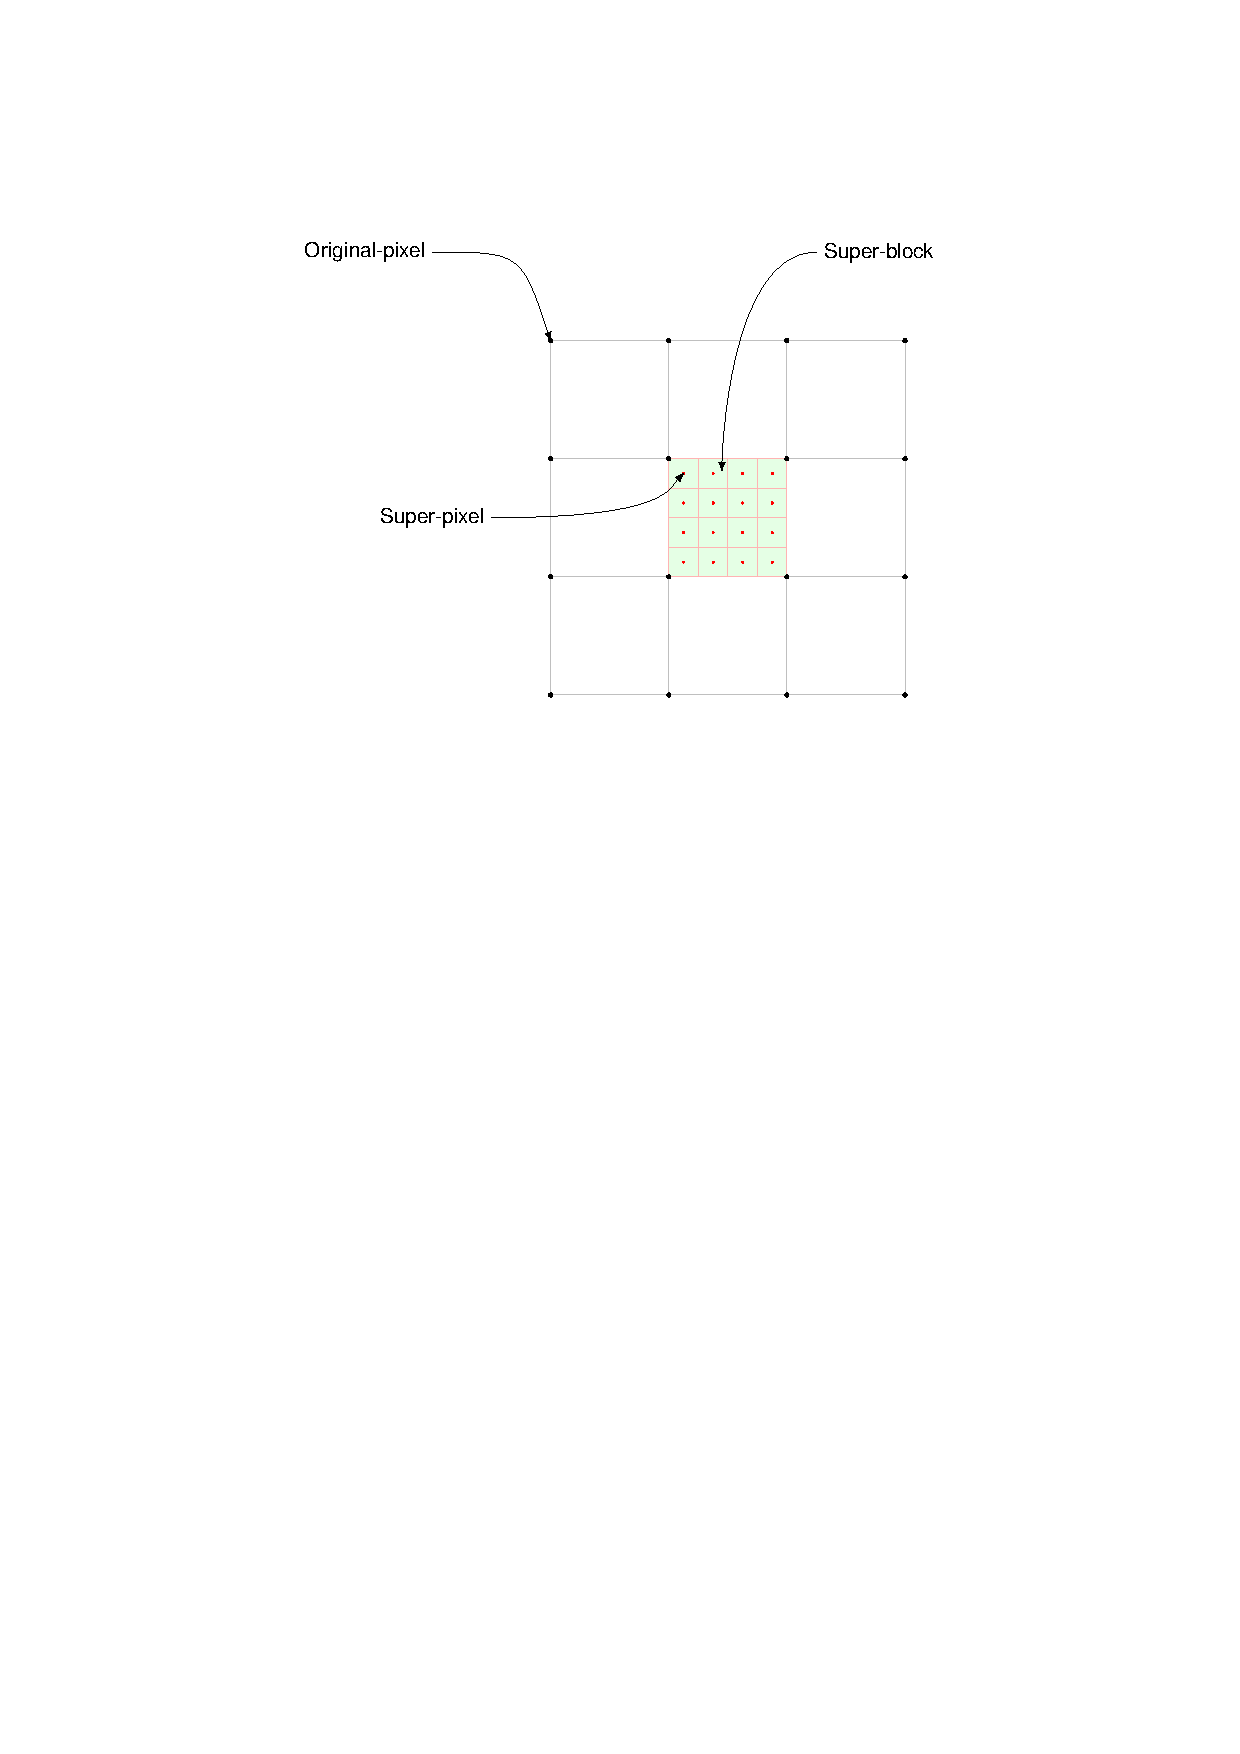
\includegraphics[scale=1]{./pic/bicubic-introduction.pdf}
		\caption{双三次插值算法简介}
		\label{bicubic_introduction}
	\end{figure}
	\par
	作为一个整体,双三次插值算法需要计算插值像素中心与原始像素中心之间的距离。使用与距离存在映射关系的双三次插值函数计算相关系数,
	然后使用该系数与原始像素点相乘,最终与 16 个原始像素点的乘积之和就是新的插值像素点结果。
	可以简单地将新插值点看作与原始像素点对应的曼哈顿距离加权,可以用式 \ref{bicubic_1} 和式 \ref{bicubic_2} 表示:
	\begin{equation}
		SP_{\vec{s}}=\sum_{\vec{o}\in{RSB}}f_B(\vert\vec{s}-\vec{o}\vert)\cdot OP_{\vec{o}}		
		\label{bicubic_1}
	\end{equation}	
	
	\begin{equation}
		f_B(|x|)=
		\begin{cases}
			(\alpha + 2)|x|^3-(\alpha+3)|x|^2+1\quad &,if\ |x| \leq1\\
			\alpha|x|^3-5\alpha|x|^2+8\alpha|x|-4\alpha\quad&,if \ 1<|x|<2\\
			0&,otherwise				
			\label{bicubic_2}
		\end{cases}
	\end{equation}
	\par
	其中,$SP_{\vec{s}}$ 为插值后像素,$\vec{s}$ 是对应的索引向量。$RSB$ 为当前插值像素所在的插值块对应的原始像素的索引集合。
	$OP_{\vec{o}}$ 为原始像素,$\vec{o}$ 是对应的索引向量。$f_B$ 则是双三次插值的核心函数。
	\par 由于双三次插值算法在我们算法设计中为预处理部分,在实现上我们着重关注在硬件设计上,并针对性的进行了大量优化,
	具体请参考文档 \href{./ref/APV21B_Algorithm_Description.pdf}{\textit{APV21B-Algorithm Description}} 介绍,此处不展开介绍。
	
	\subsection{高斯-拉普拉斯算子介绍}
	\subsubsection{概述}
	拉普拉斯算子是图像二阶空间导数的二维各向同性测度。图像的拉普拉斯算子强调快速强度变化的区域,因此经常用于边缘检测。
	拉普拉斯算子通常应用于近似高斯平滑滤波器进行平滑后的图像,以降低其对噪声的敏感性,因此这两种变体将在这里一起描述。
	该算子通常以单个灰度图像作为输入,生成另一个灰度图像作为输出。在本算法设计中,在该算子后引入一个阈值控制输出,从而实现图像二值化效果。
	\subsubsection{原理}
	记图片像素的强度值为$I(x,y)$ ,其所对应的拉普拉斯算子$L(x,y)$如式 \ref{lap} 所示:
	\begin{equation}	\label{lap}
		L(x,y)=\frac{\partial ^2 y}{\partial x^2} + \frac{\partial ^2 y}{\partial y^2}
	\end{equation}
	这个过程可以采用卷积核进行计算。由于图片是采用离散的像素值集合进行表示的,因此我们可以寻找一个近似于拉普拉斯算子的二阶导数离散卷积核。比如如下所示的两个卷积核:
	\begin{table}[h]
		\centering
		\begin{tabular}{lllll}
			\cline{1-3}
			\multicolumn{1}{|l|}{0}  & \multicolumn{1}{l|}{-1} & \multicolumn{1}{l|}{0}  &  &  \\ \cline{1-3}
			\multicolumn{1}{|l|}{-1} & \multicolumn{1}{l|}{4}  & \multicolumn{1}{l|}{-1} &  &  \\ \cline{1-3}
			\multicolumn{1}{|l|}{0}  & \multicolumn{1}{l|}{-1} & \multicolumn{1}{l|}{0}  &  &  \\ \cline{1-3}
			&                         &                         &  & 
		\end{tabular}
	\end{table}
	
	\begin{table}[h]
		\centering
		\begin{tabular}{lllll}
			\cline{1-3}
			\multicolumn{1}{|l|}{-1} & \multicolumn{1}{l|}{-1} & \multicolumn{1}{l|}{-1} &  &  \\ \cline{1-3}
			\multicolumn{1}{|l|}{-1} & \multicolumn{1}{l|}{8}  & \multicolumn{1}{l|}{-1} &  &  \\ \cline{1-3}
			\multicolumn{1}{|l|}{-1} & \multicolumn{1}{l|}{-1} & \multicolumn{1}{l|}{-1} &  &  \\ \cline{1-3}
			&                         &                         &  & 
		\end{tabular}
		\caption{近似于拉普拉斯算子的二阶导数离散卷积核}
	\end{table}
	以上的两个卷积核均可以近似为拉普拉斯算子。因为这两个卷积核都是对图片二阶导数的近似估计,它们对于图片中的噪声均很敏感。因此,为了解决这一问题,
	我们在进行拉普拉斯操作之前先对图像进行高斯平滑滤波处理,二维的高斯平滑卷积核可以用式 \ref{gauss} 进行表示。
	\begin{equation}	\label{gauss}
		G_\sigma (x,y)=\frac{1}{2\pi \sigma ^2} exp(-\frac{x^2+y^2}{2\sigma ^2}) 
	\end{equation}
	先利用高斯平滑滤波进行处理,可以降低图片中的高频噪声,方便后续的拉普拉斯操作。
	
	\subsection{高斯差分算子介绍}
	\subsubsection{概述}
	高斯差分算子 (DoG, Difference of Gaussian)\textsuperscript{\cite{14}}通过计算两个不同方差的高斯核作用于平滑同一图像的差异。从另外一个角度可以理解为,DoG 是一个可保留特定空间频率的带通滤波器,利用一个低模糊的图像与一个高模糊的图像相减完成。DoG 通过模糊处理去除掉图像中的高频噪声成分,并利用差分操作去除两图像中重叠的低频成分。通常情况下,DoG 可用于图像锐化、质量增强。
	\subsubsection{原理}
	记图片像素的强度值为 $I(x,y)$,二维的高斯平滑卷积核可参考公式 \ref{gauss},$\rho$ 作为控制图像增强比例,$\alpha$ 为高模糊高斯核的方差倍数, $G_{\sigma}(x,y)$ 表示低模糊度的高斯卷积核,$G_{\alpha\sigma}(x,y)$ 表示高模糊度的高斯卷积核算子,$D_{\sigma,\alpha,\rho}$ 表示高斯差分算子。此时可导出高斯差分函数如式 \ref{DoG} 所示。
	\begin{equation} \label{DoG}
		D_{\sigma,\alpha,\rho}(x,y)=(1+\rho)G_{\sigma}(x,y)-\rho G_{\alpha\sigma}(x,y)
	\end{equation}
	
	实际上,控制缩放因子 $\rho$ 大小,可以从在增强边缘的同时更好的保留的图像的结构特征。同时,通过级联不同方差的高斯差分算子,可以有效提取出图像中的高频、中高频、中低频信息,用于增强图像本身,提升图像质量。

	\subsection{局部二值模式介绍}
	\subsubsection{概述}
	局部二值模式 (LBP, Local Binary Pattern)\textsuperscript{\cite{8}}\textsuperscript{\cite{9}}\textsuperscript{\cite{13}} 是一种用来描述图像局部纹理特征的算子;
	它具有旋转不变形和灰度不变性等显著优点,适合用来提取图像的局部纹理特征。	
	\subsubsection{原理}
	原始的 LBP 算子\textsuperscript{\cite{13}}定义在 $3\times3$ 的窗口内,以窗口中心像素为阈值,将相邻的 8 个像素的灰度值与其进行比较,若周围像素值大于中心像素值,
	则该像素点的位置被标记为 1,否则为 0。如此,$3\times3$ 领域内的 8 个点经过比较可产生 8 位二进制数 (通常转换为十进制数即 LBP 码,共 256 种),即得到该窗口中心像素点的 LBP 值,
	并用这个值来反映该区域的纹理信息。可用公式 \ref{lbp} 来进行描述该过程。
	\begin{equation}
		LBP_{P,R}=\sum_{p=0}^{P-1}s(g_p-g_c)2^{p},\quad s(x)=\begin{cases}
			1  &,x\geq0\\
			0  &,x\le0 
		\end{cases}
		\label{lbp}
	\end{equation}
	\par
	实际上,基于原始 LBP 算子的纹理分类方法过于粗糙,对于图像区域的纹理分类有一定的局限性。
	后来出现了不少基于 LBP 改进的算法,通过引入新的参数,来获得更好的纹理分类能力。
	如圆形 LBP 算子\textsuperscript{\cite{8}}具有旋转不变性、经过统一编码 (Uniform Pattern) 后对算子种类进行降维,
	CLBP 算子\textsuperscript{\cite{9}}引入图像的局部梯度参数以增强纹理分类能力。

	\section{算法优化}
	通过上节我们可以看到,RAISR 作者对于滤波器的学习以及应用进行了不少的优化,但是对于我们将该算法应用到硬件实现上,有着不小的挑战。第一个是在于,每个像素类型需要学习 216 个滤波器,
	而对于进行 4 倍上采样的整幅图像可分为 16 种类型,总共就需要 3456 个滤波器进行片上存储。在 FPGA 上存储如此大量的数据是不划算的。
	第二点是,为了能获得像素更多的信息,RAISR 采用了 $11\times11$ 大小的滤波器进行卷积,这对于硬件资源消耗量极大,
	在考虑量化同时保留运算过程中数据合适位宽并满足运算时延,每个像素进行锐化操作至少需要 180 个 DSP 进行乘累加运算(不考虑硬件复用以减少资源消耗),总延时至少 12 个时钟周期输出延迟,该结果已经考虑了使用树形结构对数据进行运算。
	第三点,哈希表键的运算不仅需要进行除法、开方及反正切运算,还需要进行奇异值分解,这对于 FPGA 实时性设计要求难度提升了一个等级。
	\subsection{概述}
	我们提出了一个创新的 \textbf{LBP-RAISR} 算法,以 \textbf{RAISR} 为主体框架,整体上分为了三个阶段。
	第一步,通过双三次插值算法\textsuperscript{\cite{4}\cite{5}},将 LR 图像映射到 HR 图像上,得到最终需要的目的分辨率图像 Pre-SR;
	第二步,对图像以每个像素为中心进行 $5\times5$ 分块,遍历 Pre-HR 图像的每一个图像块,
	进行高斯-拉普拉斯(LoG)纹理检测后使用 CLBP 算法\textsuperscript{\cite{8}\cite{9}}结合角度信息求解进行纹理分类。
	显而易见,这里我们的设计与 \textbf{RAISR} 有较大的区别,这是出于对硬件设计的考量,具体的设计细节会在下一节和 RTL设计文档 中详细解释。
	第三步,利用上一步的得到每个图像块的类型找到对应的滤波器,作用于图像块进行卷积,得到更接近于原始 HR 的像素,最后得到更高质量的 SR 图像。
	整体框架如图\ref{overview}所示。
	\begin{figure}[h]
		\centering
		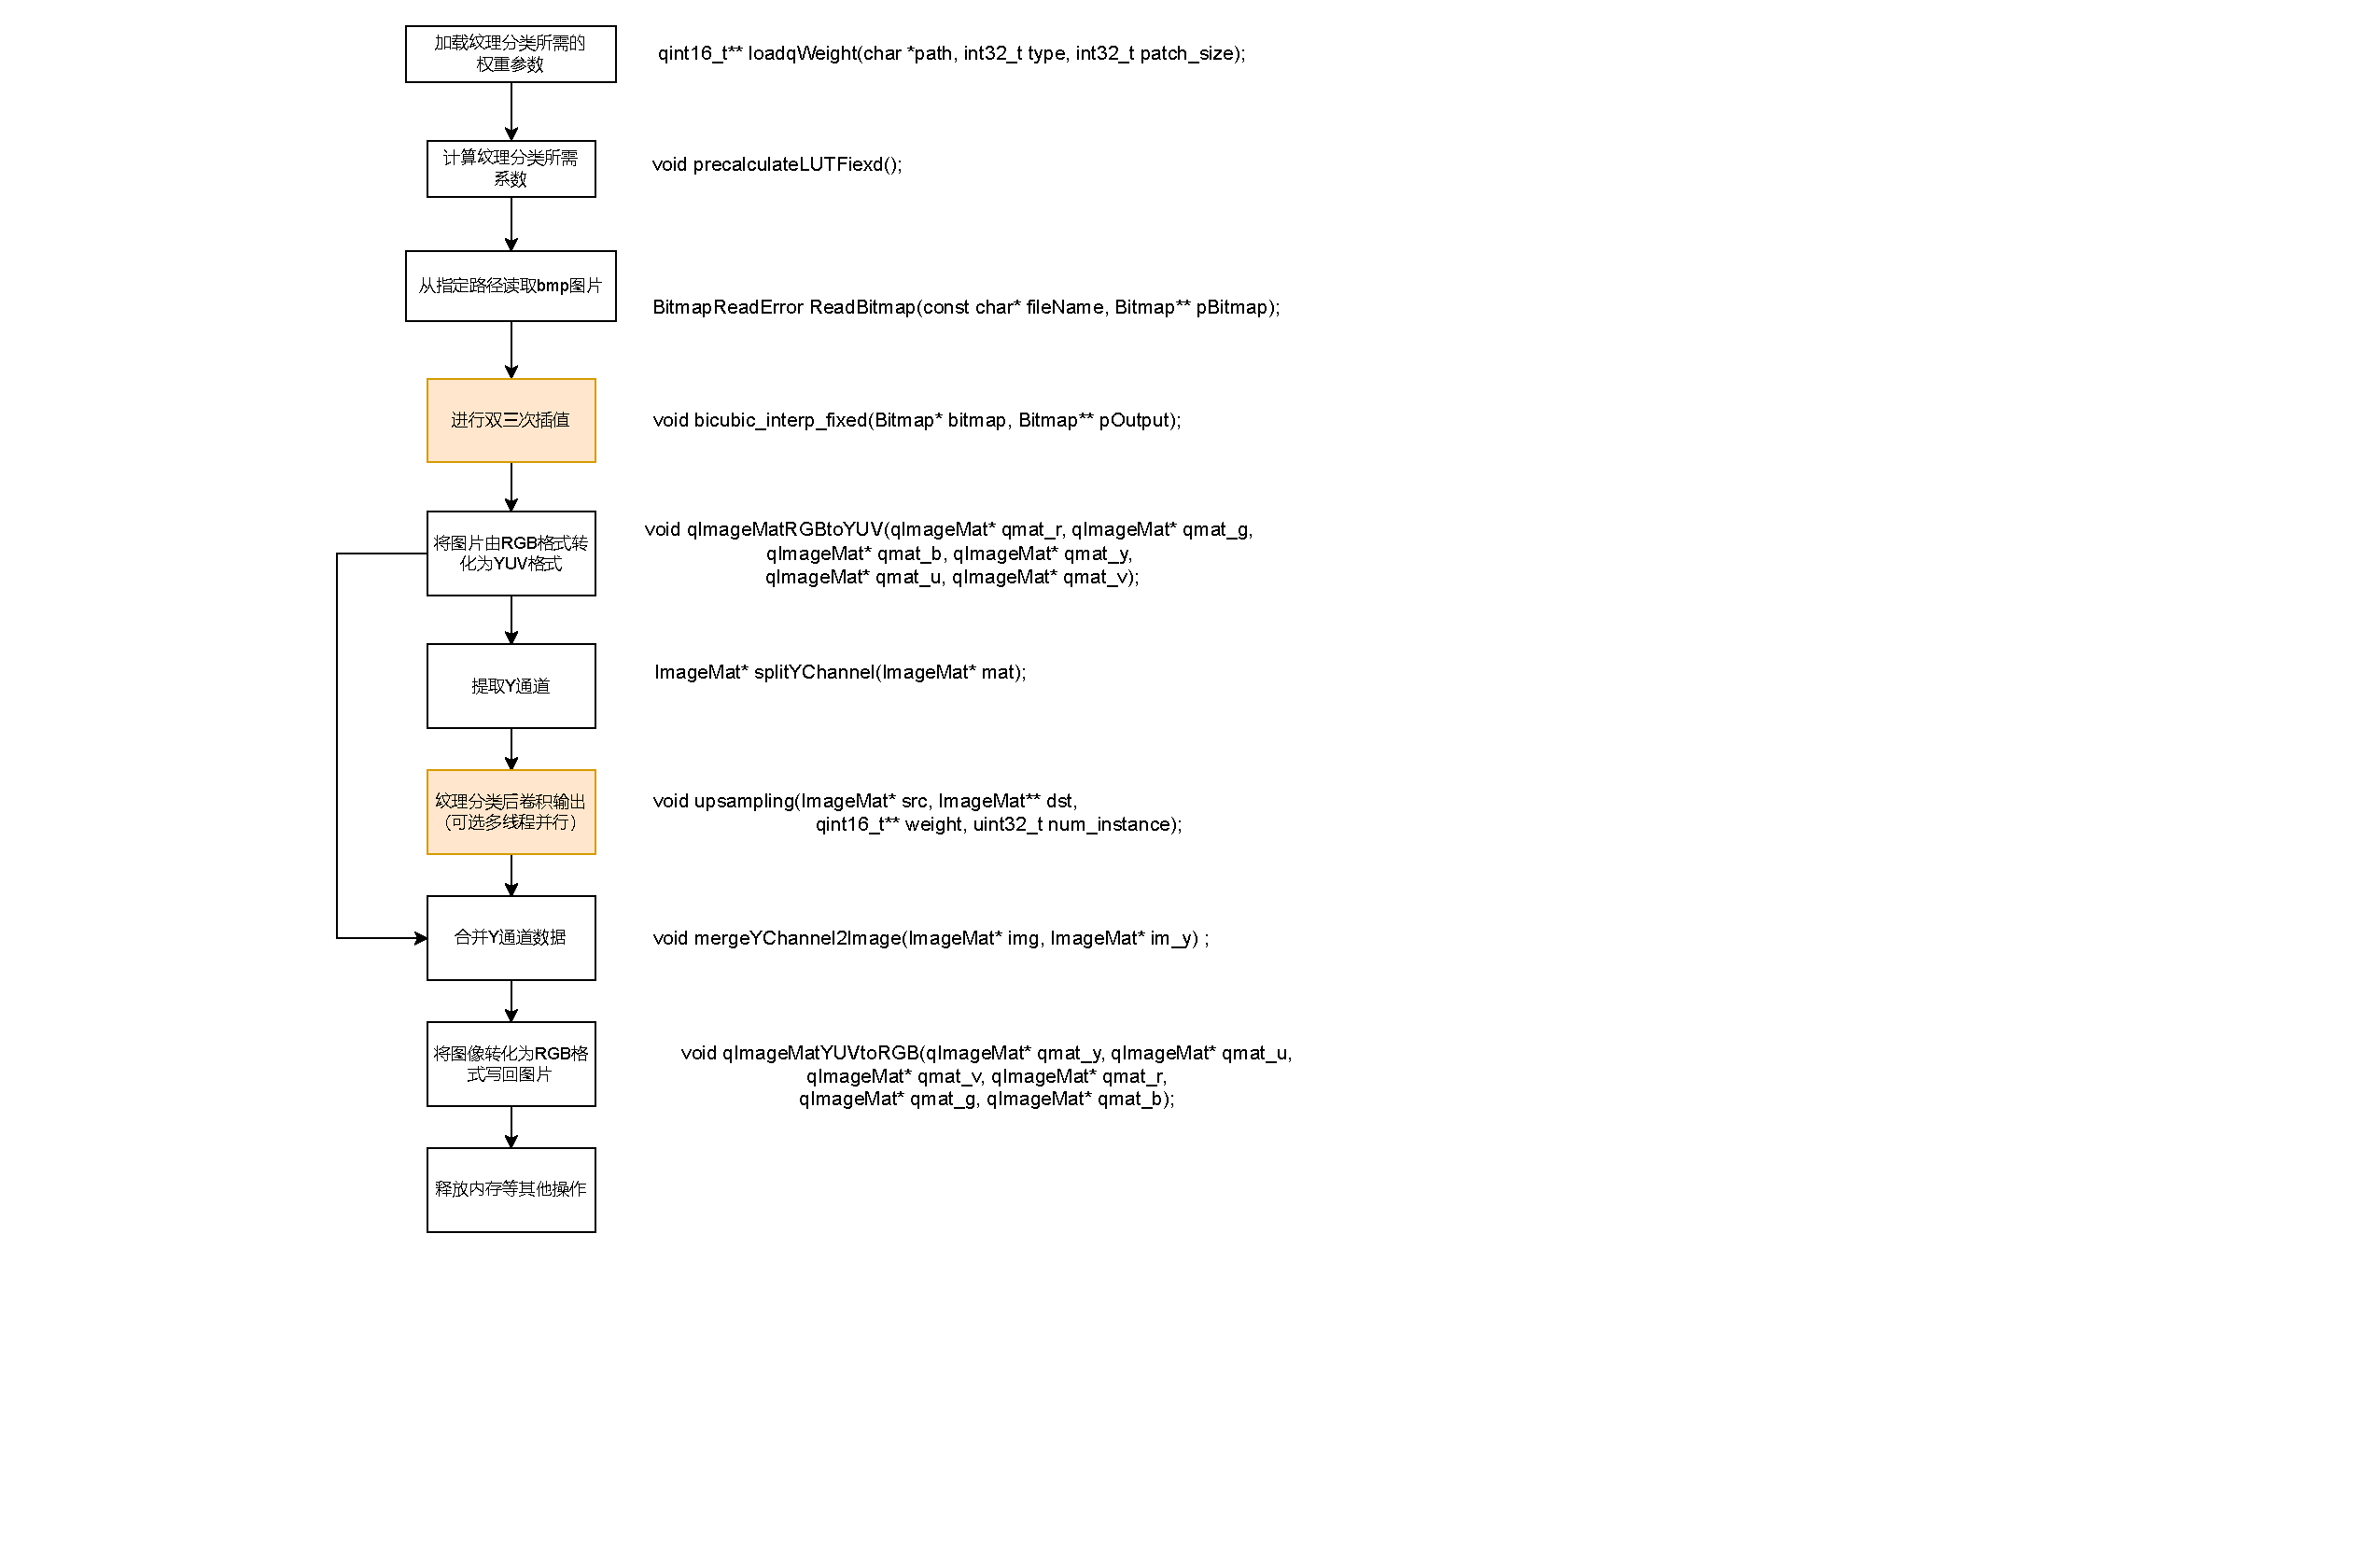
\includegraphics[scale=0.72]{./pic/overview.pdf}
		\caption{算法架构}
		\label{overview}
	\end{figure}
	\subsection{实现步骤}
	\subsubsection{双三次插值}
	作为第一步,我们需要将 LR 图像先上采样到需要的分辨率,可以使用传统的插值方法如最近邻插值、双线性插值、双三次插值、Lanczos 插值等算法。
	由于考虑到上采样图片的质量效果会应影响到最终的高分辨率图片质量与运算过程中的尽可能降低复杂度,双三次插值成为了我们算法预处理的最优选择。
	\subsubsection{纹理分类}
	我们对经过 4 倍上采样后的 Pre-SR 图片先进行高斯-拉普拉斯滤波(LoG)\textsuperscript{\cite{12}},然后给定一个阈值区间对进行滤波后的像素值进行二值化操作,
	采用 CLBP 算法对二值化后的图像纹理进行按块分类。这里需要注意的是,我们采用 $5 \times 5$ 的图像块进行纹理分类,由于已经对图像块进行了纹理检测这一步操作,
	所以 CLBP 算法步骤我们并没有严格执行,保留 $C$ 中心像素与 $u$ 统一编码这两个参数。考虑到该算法需要对圆形区域检测需要进行三角函数进行运算,
	我们将其近似等效为最外边缘的二值像素,从而减轻运算量。但是 CLBP 算法经过统一编码后具有旋转不变形,与滤波器需要学习局部纹理方向角度特征相矛盾,
	故此我们增加了一步操作,当进行对像素统一编码时,保留了角度信息,从而增加选择滤波器参数条件。此时,纹理分类结束。
	\subsubsection{卷积输出}
	在上一步中我们已经通过纹理分类得到了图像块的纹理类型,根据这个类型我们可以选择预学习的滤波器,对相应的 Pre-SR 图像块进行卷积操作,从而得到了 SR 像素,最终输出 SR 图像。
	
	\chapter{效果展示}
	我们将提出的算法与 RAISR 进行了对比,	其中 Set5 是单帧图像超分辨率任务中最常用的数据集,GameSet 是景嘉微在本次杯赛中提供的测试效果图片。
	
	\begin{figure}[h]
		\centering
		\subfigure[GT]{
			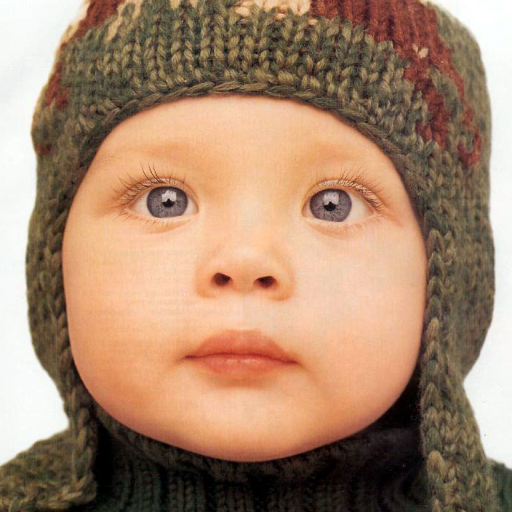
\includegraphics[scale=0.35]{./pic/GT-1.png}
		}
		\quad
		\subfigure[bicubic]{
			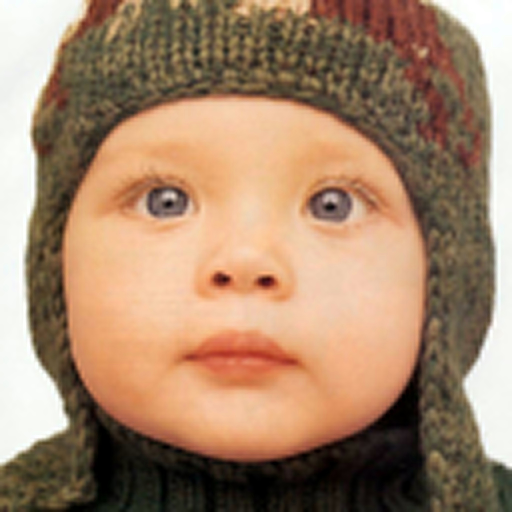
\includegraphics[scale=0.35]{./pic/bicubic-1.png}
		}
		\quad
		\subfigure[raisr]{
			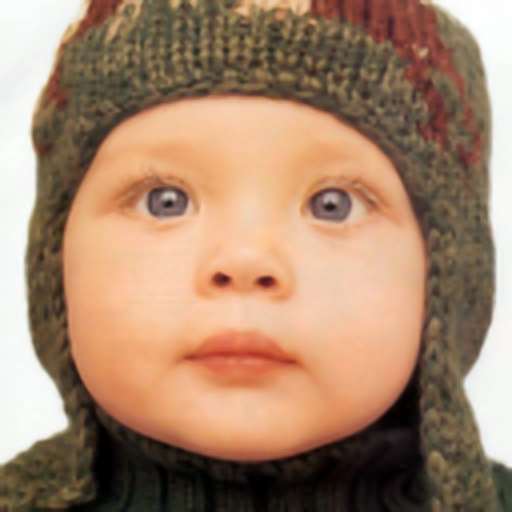
\includegraphics[scale=0.35]{./pic/raisr-1.png}
		}
		\quad
		\subfigure[lbp-raisr]{
			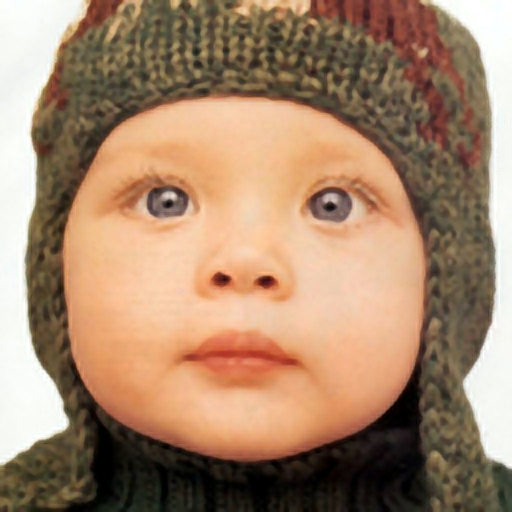
\includegraphics[scale=0.35]{./pic/lbp-raisr-1.png}
		}
		\caption{各算法实现效果对比-例1}
	\end{figure}
	
	\begin{figure}[h]
		\centering
		\subfigure[GT]{
			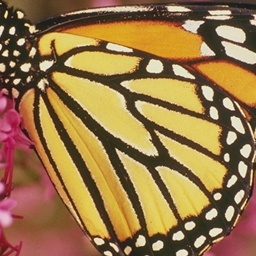
\includegraphics[scale=0.7]{./pic/GT-2.png}
		}
		\quad
		\subfigure[bicubic]{
			
\includegraphics[scale=0.7]{./pic/bicubic-2.png}
		}
		\quad
		\subfigure[raisr]{
			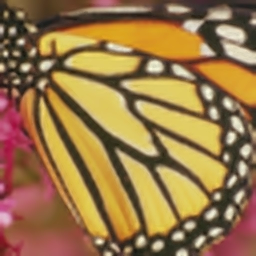
\includegraphics[scale=0.7]{./pic/raisr-2.png}
		}
		\quad
		\subfigure[lbp-raisr]{
			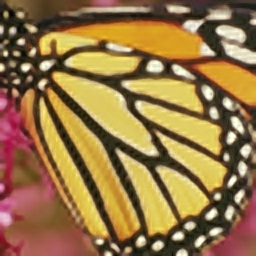
\includegraphics[scale=0.7]{./pic/lbp-raisr-2.png}
		}
		\caption{各算法实现效果对比-例2}
	\end{figure}
	
	
	%	\newcounter{Rownumber}
	%	\newcommand{\Rown}{\stepcounter{Rownumber}\theRownumber}
	\begin{table}[htb]
		\small
		\begin{tabular}{|c|c|c|c|c|c|c|}
			\hline
			\textbf{DataSet} & \textbf{Scale} & \textbf{Bilinear} & \textbf{Bicubic} & \textbf{RAISR} & \textbf{LBP-RAISR} & \textbf{\begin{tabular}[c]{@{}c@{}}LBP-RAISR\\ (Quantized)\end{tabular}} \\ \hline
			Set5(PSNR)       & x4             & 25.79             & 26.84            & 27.05          & \textbf{27.61}     & \textbf{27.61}\\ \hline
			Set5(SSIM)       & x4             & 0.765             & 0.790            & 0.803          & 0.812     			& \textbf{0.817}                                                                    \\ \hline
			Set5(LPIPS)      & x4             & 0.335             & 0.310            & 0.269          & \textbf{0.198}     & 0.200                                                                    \\ \hline
			GameSet(PSNR)    & x4             & 30.83             & 31.51            & 31.59          & \textbf{32.02}     & 32.00                                                                    \\ \hline
			GameSet(SSIM)    & x4             & 0.847             & 0.862            & 0.861          & 0.870     		& \textbf{0.871}                                                                    \\ \hline
			GameSet(LPIPS)   & x4             & 0.288             & 0.265            & 0.263          & \textbf{0.209}     & 0.211                                                                    \\ \hline
		\end{tabular}
		\caption{各算法实现评分对比}
	\end{table}

	
	\chapter{团队及指导老师介绍}
	\section{团队介绍}
	\subsubsection{黄金源}
	黄金源,男,来自深圳大学电子与信息工程学院大三年级通信工程专业,FPGA 及数字集成电路设计方向,本科期间曾多次参加电子设计和FPGA相关竞赛,并取得不错成绩,同时对于高级体系结构设计有着浓厚兴趣。
	\subsubsection{邓立唯}
	邓立唯,男,来自广西南宁,现大三,就读于中国计量大学微电子科学与工程专业,数字集成电路设计方向。\par
	从小热爱计算机技和电子技术,初中时就掌握了单片机的开发,从那时起,就梦想着有朝一日能创造出属于自己的芯片。自高中认识 FPGA来,学习了很多 FPGA 开发技术,并逐渐将研究重心转移到数字集成电路开发上来,学习并掌握了很多业内的现代化集成电路设计流程和方法,并利用FPGA没计了数个商业项目的核心控制器和 IP,具有一定的工程实践经历。\par
	\subsubsection{林明锋}
	林明锋,男,来自深圳大学电子与信息工程学院大三年级微电子科学与工程专业,嵌入式设计方向,对数字集成电路设计有浓厚兴趣。
	
	\section{指导老师介绍}
	\subsubsection{邓磊}
	邓磊,现为深圳大学电子与信息工程学院丁文华院士团队助理教授。2012年于上海交通大学信息工程系获学士学位,2017于香港中文大学信息工程系获博士学位,2015年于美国普渡大学电子与计算机工程学院任访问学者。其研究兴趣包括数字创意技术与装备,具有严格时延要求的通信网络,以及智能交通系统。其研究工作已发表在 ACM SIGMETRICS, IEEE INFOCOM和ACM e-Energy 等国际顶级会议以及 IEEE/ACM Transactions on Networking, IEEE Journal on Selected Areas in Communications和IEEE Transactions on Intelligent Transportation Systems 等国际著名期刊上,详情请参看其个人主页 https://leideng.github.io/。
	
	\subsubsection{唐莹}
	唐莹,女,1988年出生,湖南永州人,工学博士,副研究员。主持/参加国家和省部级项目8项,其中主持国家自然科学基金 1 项,广西自然科学基金2项,区级研究生教改项目1项。近五年来,在 Journal of the European Ceramic Society、Ceramics International、Journal of Alloys and Compounds、J Mater Sci: Mater Electron、Journal of the American Ceramic Society、Materials Letters 等国际主流期刊发表相关研究论文30余篇,其中以第一作者及通讯作者在 SCI 一区发表 19 篇论文。工作以来已获得授权中国发明专利 20 余项。\par 主要研究方向:电子信息功能材料 \par 联系方式:广西省桂林市建干路12号桂林理工大学理学院(邮编:541004)\par 邮箱:tangyinggl001@aliyun.com
	
	
	
	%参考文献		
\newpage
\begin{thebibliography}{99}
\bibitem{1}Romano, Yaniv, John Isidoro, and Peyman Milanfar. "RAISR: rapid and accurate image super resolution." IEEE Transactions on Computational Imaging 3.1 (2016): 110-125.
\bibitem{2}Jeong, S. C.; Song, B. C. Training-based superresolution algorithm using k-means clustering and detail enhancement. In: Proceedings of the 18th European Signal Processing Conference, 1791–1795, 2010.
\bibitem{3} Yu, G. S.; Sapiro, G.; Mallat, S. Solving inverse problems with piecewise linear estimators: From Gaussian mixture models to structured sparsity. IEEE Transactions on Image Processing Vol. 21, No. 5, 2481–2499, 2012
\bibitem{4}R.G. Keys, "Cubic convolution interpolation for digital image processing," IEEE Transaction on Acoustics, Speech and Signal processing, vol. 29, no. 6, Dec. 1981, pp. 1153-1160.
\bibitem{5}H.S. Hou and H.C. Andrews, "Cubic splines for image interpolation and digital filtering," IEEE Transaction Signal processing, vol. 26, no. 6, Dec. 1978, pp. 1153-1160.
\bibitem{6}X. Feng and P. Milanfar, "Multiscale principal components analysis for image local orientation estimation," Proceedings of the 36th Asilomar Conference on Signals, Systems and Computers, Pacific Grove, CA, November 2002. 5
\bibitem{7}Zabih, R.; Woodfill, J. Non-parametric local transforms for computing visual correspondence. In: Computer Vision — ECCV '94. Lecture Notes in Computer Science, Vol. 801. Eklundh, J. O. Ed. Springer Berlin Heidelberg, 151–158, 1994.
\bibitem{8}T. Ojala, M. Pietikainen and T. Maenpaa, "Multiresolution gray-scale and rotation invariant texture classification with local binary patterns," in IEEE Transactions on Pattern Analysis and Machine Intelligence, vol. 24, no. 7, pp. 971-987, July 2002, doi: 10.1109/TPAMI.2002.1017623.
\bibitem{9}Z. Guo, L. Zhang and D. Zhang, "A Completed Modeling of Local Binary Pattern Operator for Texture Classification," in IEEE Transactions on Image Processing, vol. 19, no. 6, pp. 1657-1663, June 2010, doi: 10.1109/TIP.2010.2044957.
\bibitem{10} R. Keys, "Cubic convolution interpolation for digital image processing," IEEE Trans. on Acoustics, Speech and Signal Proc., vol. 29, no. 6, pp. 1153–1160, 1981. 1
\bibitem{11}H. Hou and H. Andrews, "Cubic splines for image interpolation and digital filtering," IEEE Trans. on Acoustics, Speech and Signal Proc., vol. 26, no. 6, pp. 508–517, 1978. 1
\bibitem{12}Marr D, Hildreth E. Theroy of edge detection. Proc. of the Royal Society of London. Series B. Biological Sciences, 1980,207(1167): 187-217.
\bibitem{13}Ojala, T., Pietikäinen, M. and Harwood, D. (1996), A Comparative Study of Texture Measures with Classification Based on Feature Distributions. Pattern Recognition 19(3):51-59.
\bibitem{14}D. Marr and E. Hildreth, “Theory of edge detection,” Proceedings of the Royal Society of London B: Biological Sciences, vol. 207, no. 1167, pp. 187–217, 1980. 2

\end{thebibliography}
	
	
	
	
\end{document}




	
	
